\thispagestyle{plain}
\noindent It was stated in the project description that we shoud use a nois that was given by
the normal distribution $\mathcal{N}(0,1)$. What we found was that since the Franke
Function when plotten for $x$ and $y$ in the range between $0$ and $1$ the maximal 
value of the Franke function becomes around $1.4$. When plottet with noise that had values
between $0$ and $1$ the plot of the franke function becomes unrecognizable as shown in figure \eqref{franke noise 1}. 
\begin{figure}[H]
	\centering
	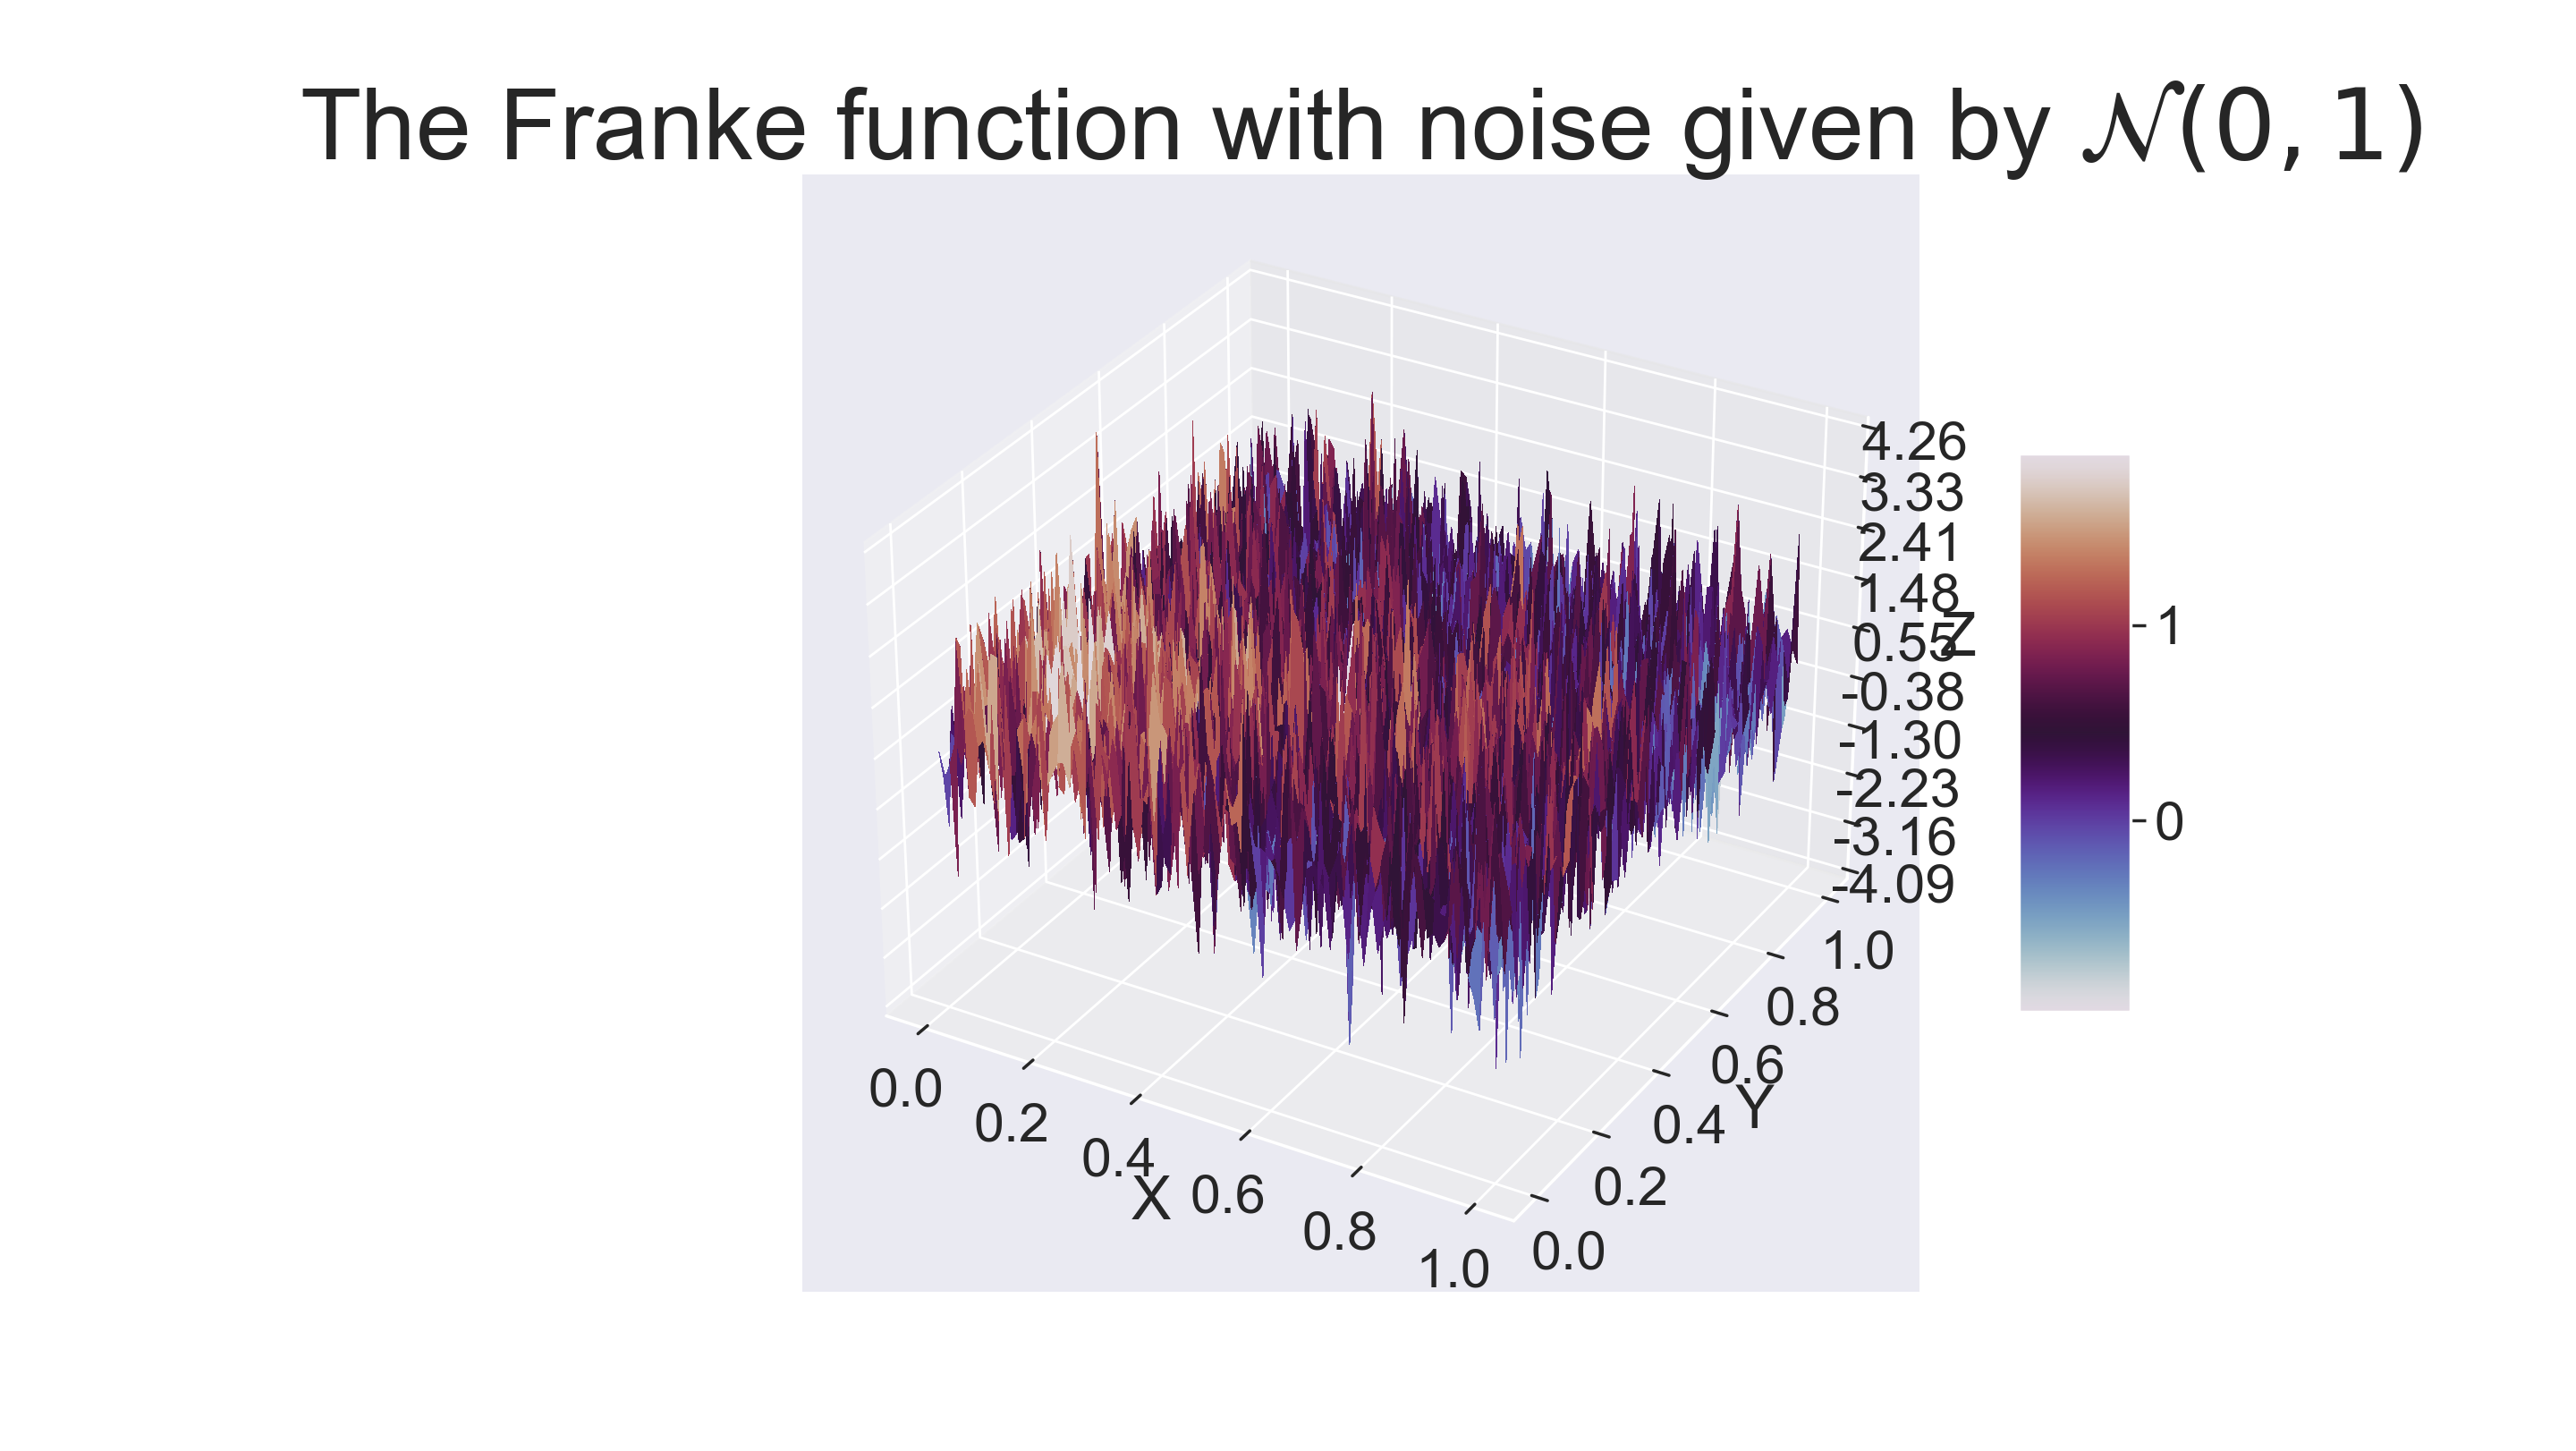
\includegraphics[width=0.5\textwidth]{Figure_13.png}
	\caption{Plot showing the Frankece function with noise given by the normal distrubution $\mathcal{N}(0,1)$ }
	\label{franke noise 1}
\end{figure}
\noindent But if instead the normal distribution $\mathcal{N}(0,0.1)$ is 
used, the dataset becomes much easier to work with, and the results becomes 
much prettier (as shown in figure \eqref{franke noise 0.1}) since noise has a tendency of ruining everything.
\begin{figure}[H]
	\centering
	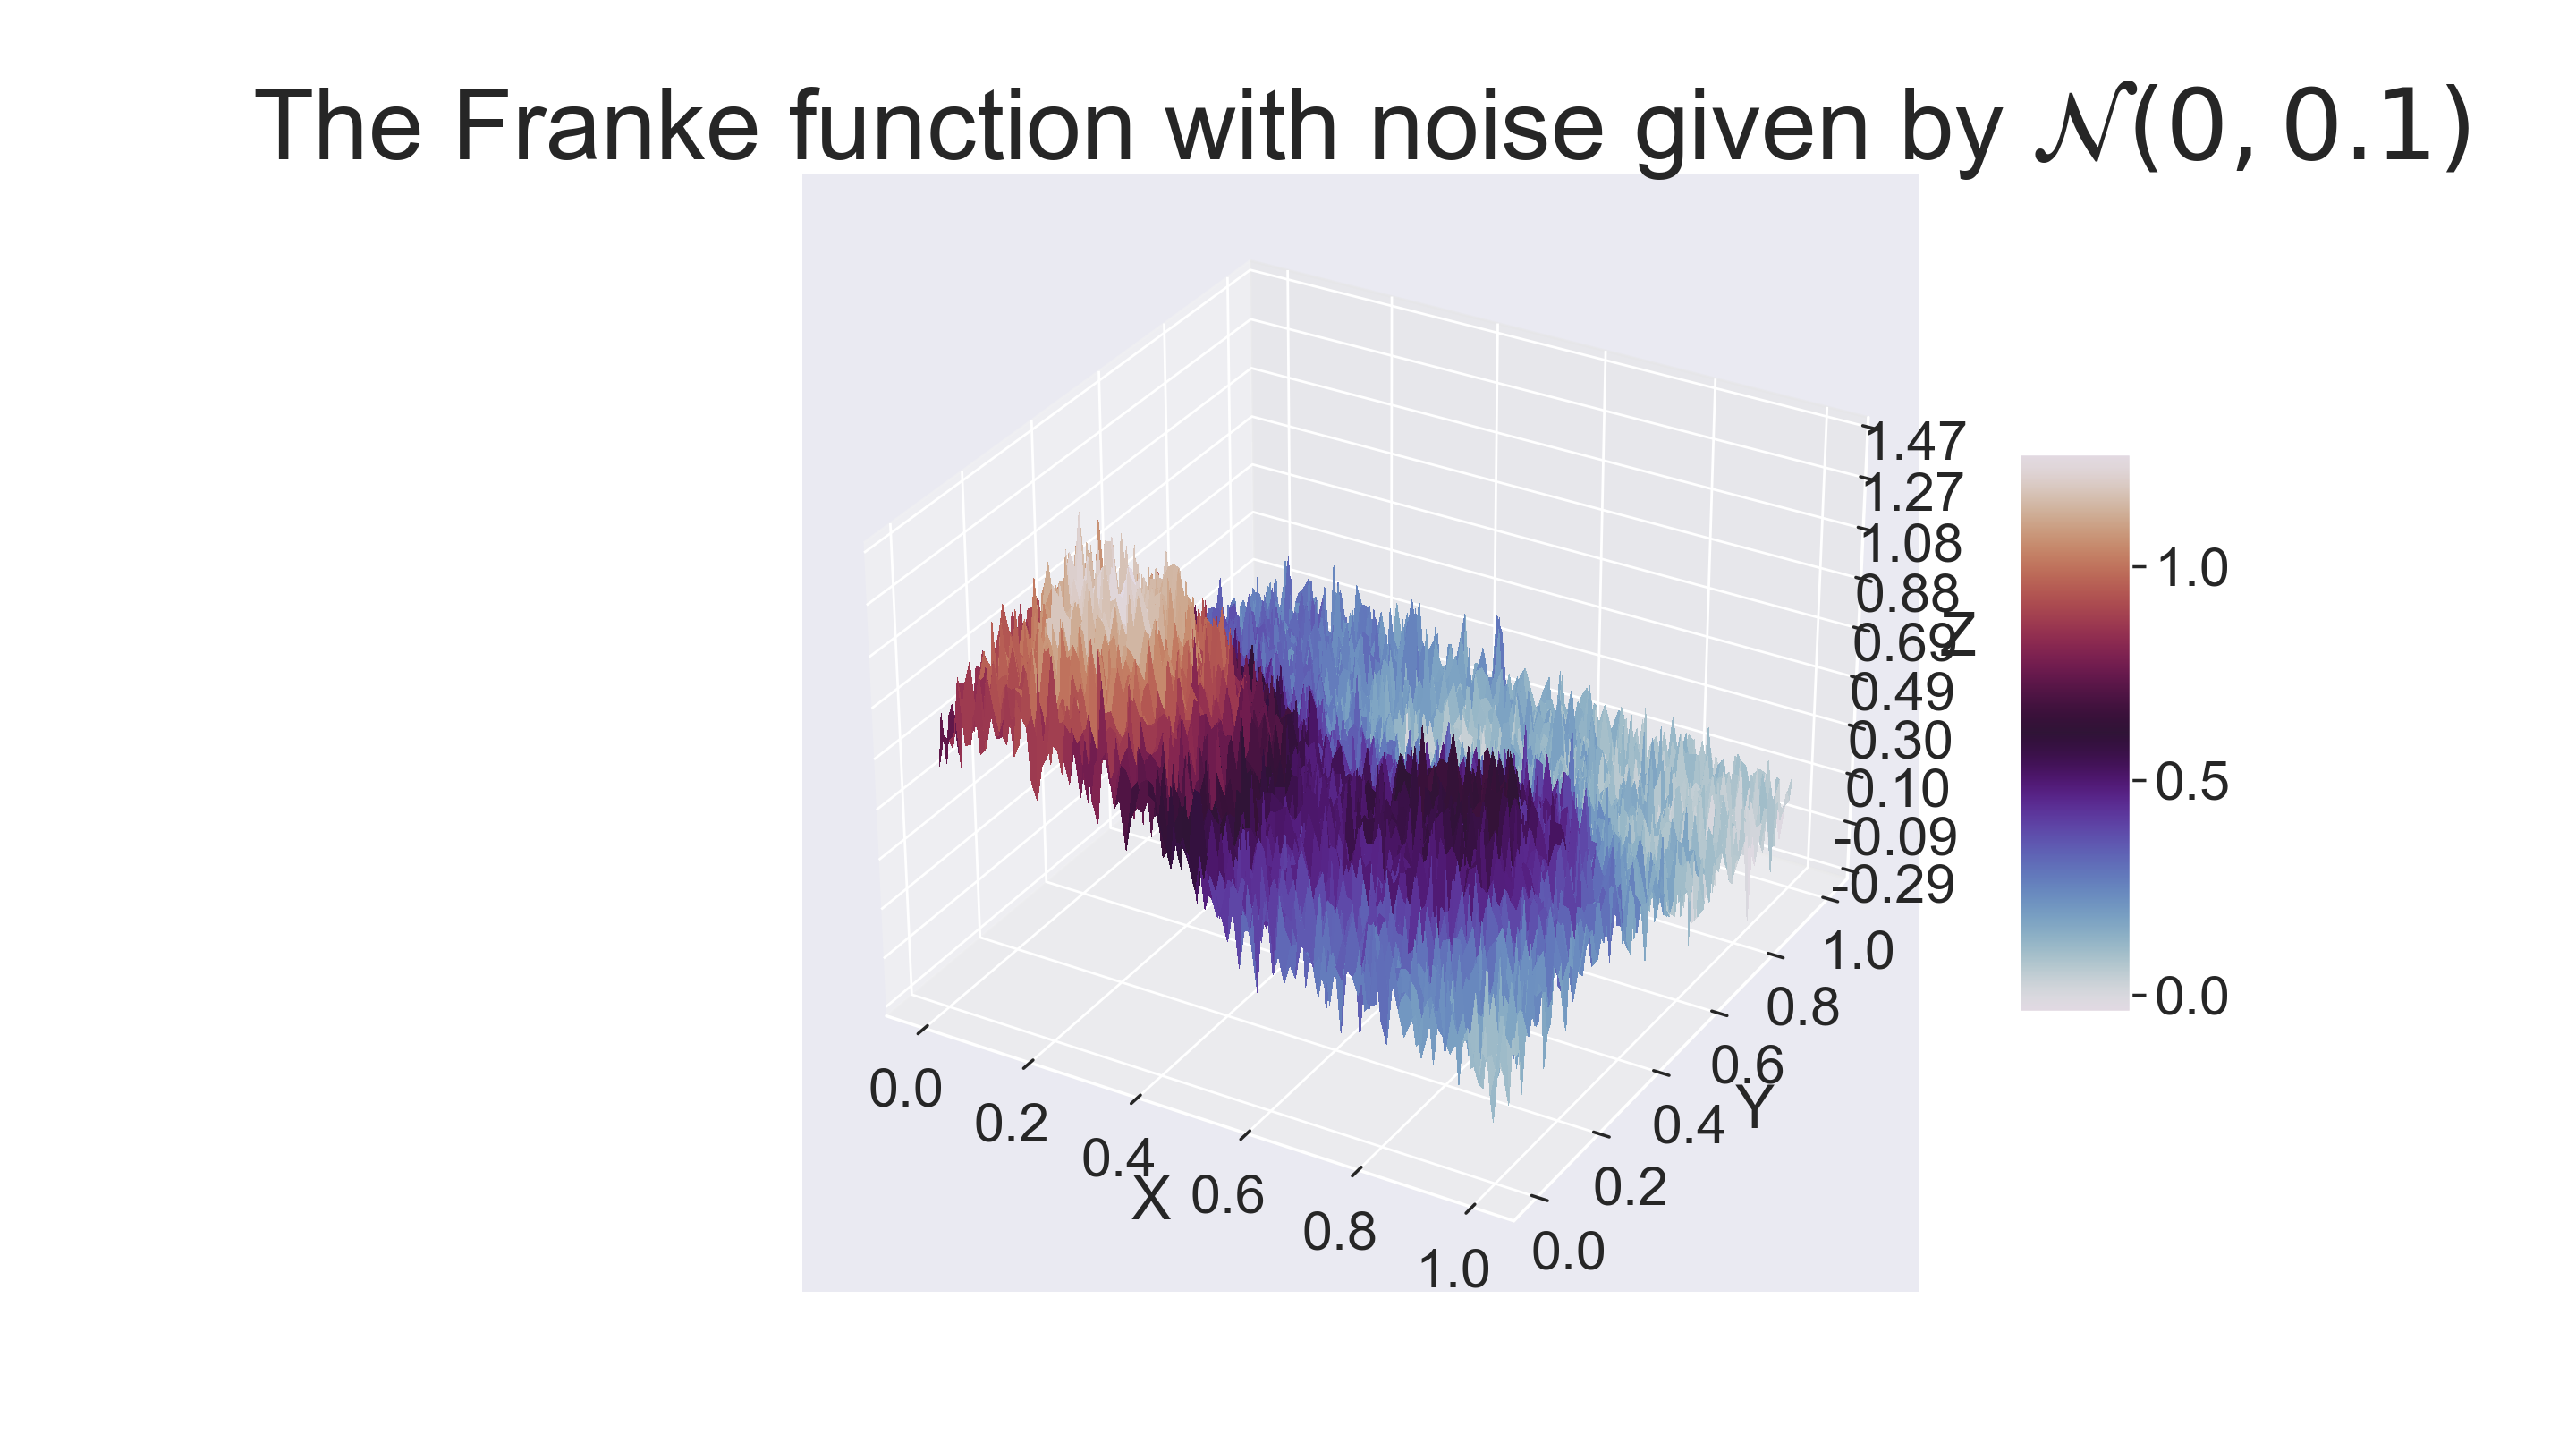
\includegraphics[width=0.5\textwidth]{Figure_14.png}
	\caption{Plot showing the Frankece function with noise given by the normal distrubution $\mathcal{N}(0,0.1)$ }
	\label{franke noise 0.1}
\end{figure}
\noindent Now that we have gotten that out of the way, we can start actually
discussing the result of the regression analysis of the Franke function.

\subsection*{The Franke function}
\noindent Since the parameter x and y only had values from 0 to 1 when creating the 
Franke function we did not see it necessary to scale the data.

\noindent From figure \eqref{MSE and R2 OLS} we see that when our data set does not include noise
the MSE for the training data gets lower with increas in complexity, while 
the R2 score gets closer and closer to 1. But when we introduce noise whe see from figure \eqref{MSE and R2 OLS noise}
that for our test data the MSE acctually increase with higher complexity. 

The dataset containing the test data consists of $20\%$ of the original
dataset. This implies that the number of points in the test data is 
significantly smaller than that in the training data. We anticipate 
that by increasing the number of data points, the MSE for the model 
created using the test data will converge towards that of the training
model.

What we can see from figure \eqref{beta OLS} is that for the higher order 
polynomials the values for the coefficients varies a lot in value. This is due to 
the regression method trying to fit the function to the noise, so this is a direct 
effect of overfitting the function with a to high order polynomial. From figure \eqref{beta OLS}
we see that the beta values start to vary at as low as a fourth order polynomial and that 
for a fifth order polynomial the variance start to become substantially large. This is 
also supported by the MSE plot shown in figure \eqref{MSE and R2 OLS noise}, where we can
see that the MSE starts to gradually increase after the third order polynomial. So we clearly
start to move in to the overfit area. 

We expect that if we set $\lambda = 0$ in our Ridge regression then the result 
will be the same as for OLS. From figur .. and ... we se that when lambda is 
set to zero then the model becoms equal to that for OLS, explenation...


\subsection*{Real terrain data}